\documentclass[a4paper,twoside,12pt]{article}
%\usepackage [reqno] {amsmath}
\usepackage{amsfonts,amstext}
\usepackage{amsmath}
\usepackage{german}
\usepackage{graphicx}
\usepackage{fullpage}

\newcommand{\ZETTELNUMMER}{4}

\newcounter{AUFGNR}
\setcounter{AUFGNR}{1}
\newcommand{\AUFGABE}[2]{\vspace{0.3cm}\item[Aufgabe~\arabic{AUFGNR}]\stepcounter{AUFGNR} #1\hfill\emph{#2}}


\newcommand{\floor}[1]{\left\lfloor{#1}\right\rfloor}
\newcommand{\ceil}[1]{\left\lceil{#1}\right\rceil}
\newcommand{\half}[1]{\frac{#1}{2}}
\newcommand{\N}{\mathbb{N}}



\renewcommand{\labelenumi}{(\alph{enumi})}
\renewcommand{\labelenumii}{(\roman{enumii})}


\begin{document}
\pagestyle{empty}
\hrule\medskip
\rule{0ex}{0ex}\\[-1ex]
\ZETTELNUMMER. Aufgabenblatt zur Vorlesung

\smallskip
\noindent
\large
\textbf{Nichtsequentielle und Verteilte Programmierung}\hfill SoSe
2018 \\[0.5ex]
\normalsize
Anton Oehler, Mark Niehues

\newcommand{\immer}{\Box}
\newcommand{\irgendwann}{\lozenge}
\newcommand{\folgt}{\Rightarrow}
\newcommand{\oder}{\vee}
\newcommand{\und}{\wedge}

\medskip\hrule

\begin{description}
% Aufgabe 1
\AUFGABE{Lineare Temporale Logik I}{10 Punkte}
\begin{enumerate}
  \item { \[
     \lozenge \Box\, p \Leftrightarrow \Box \lozenge\, p
  \]}

  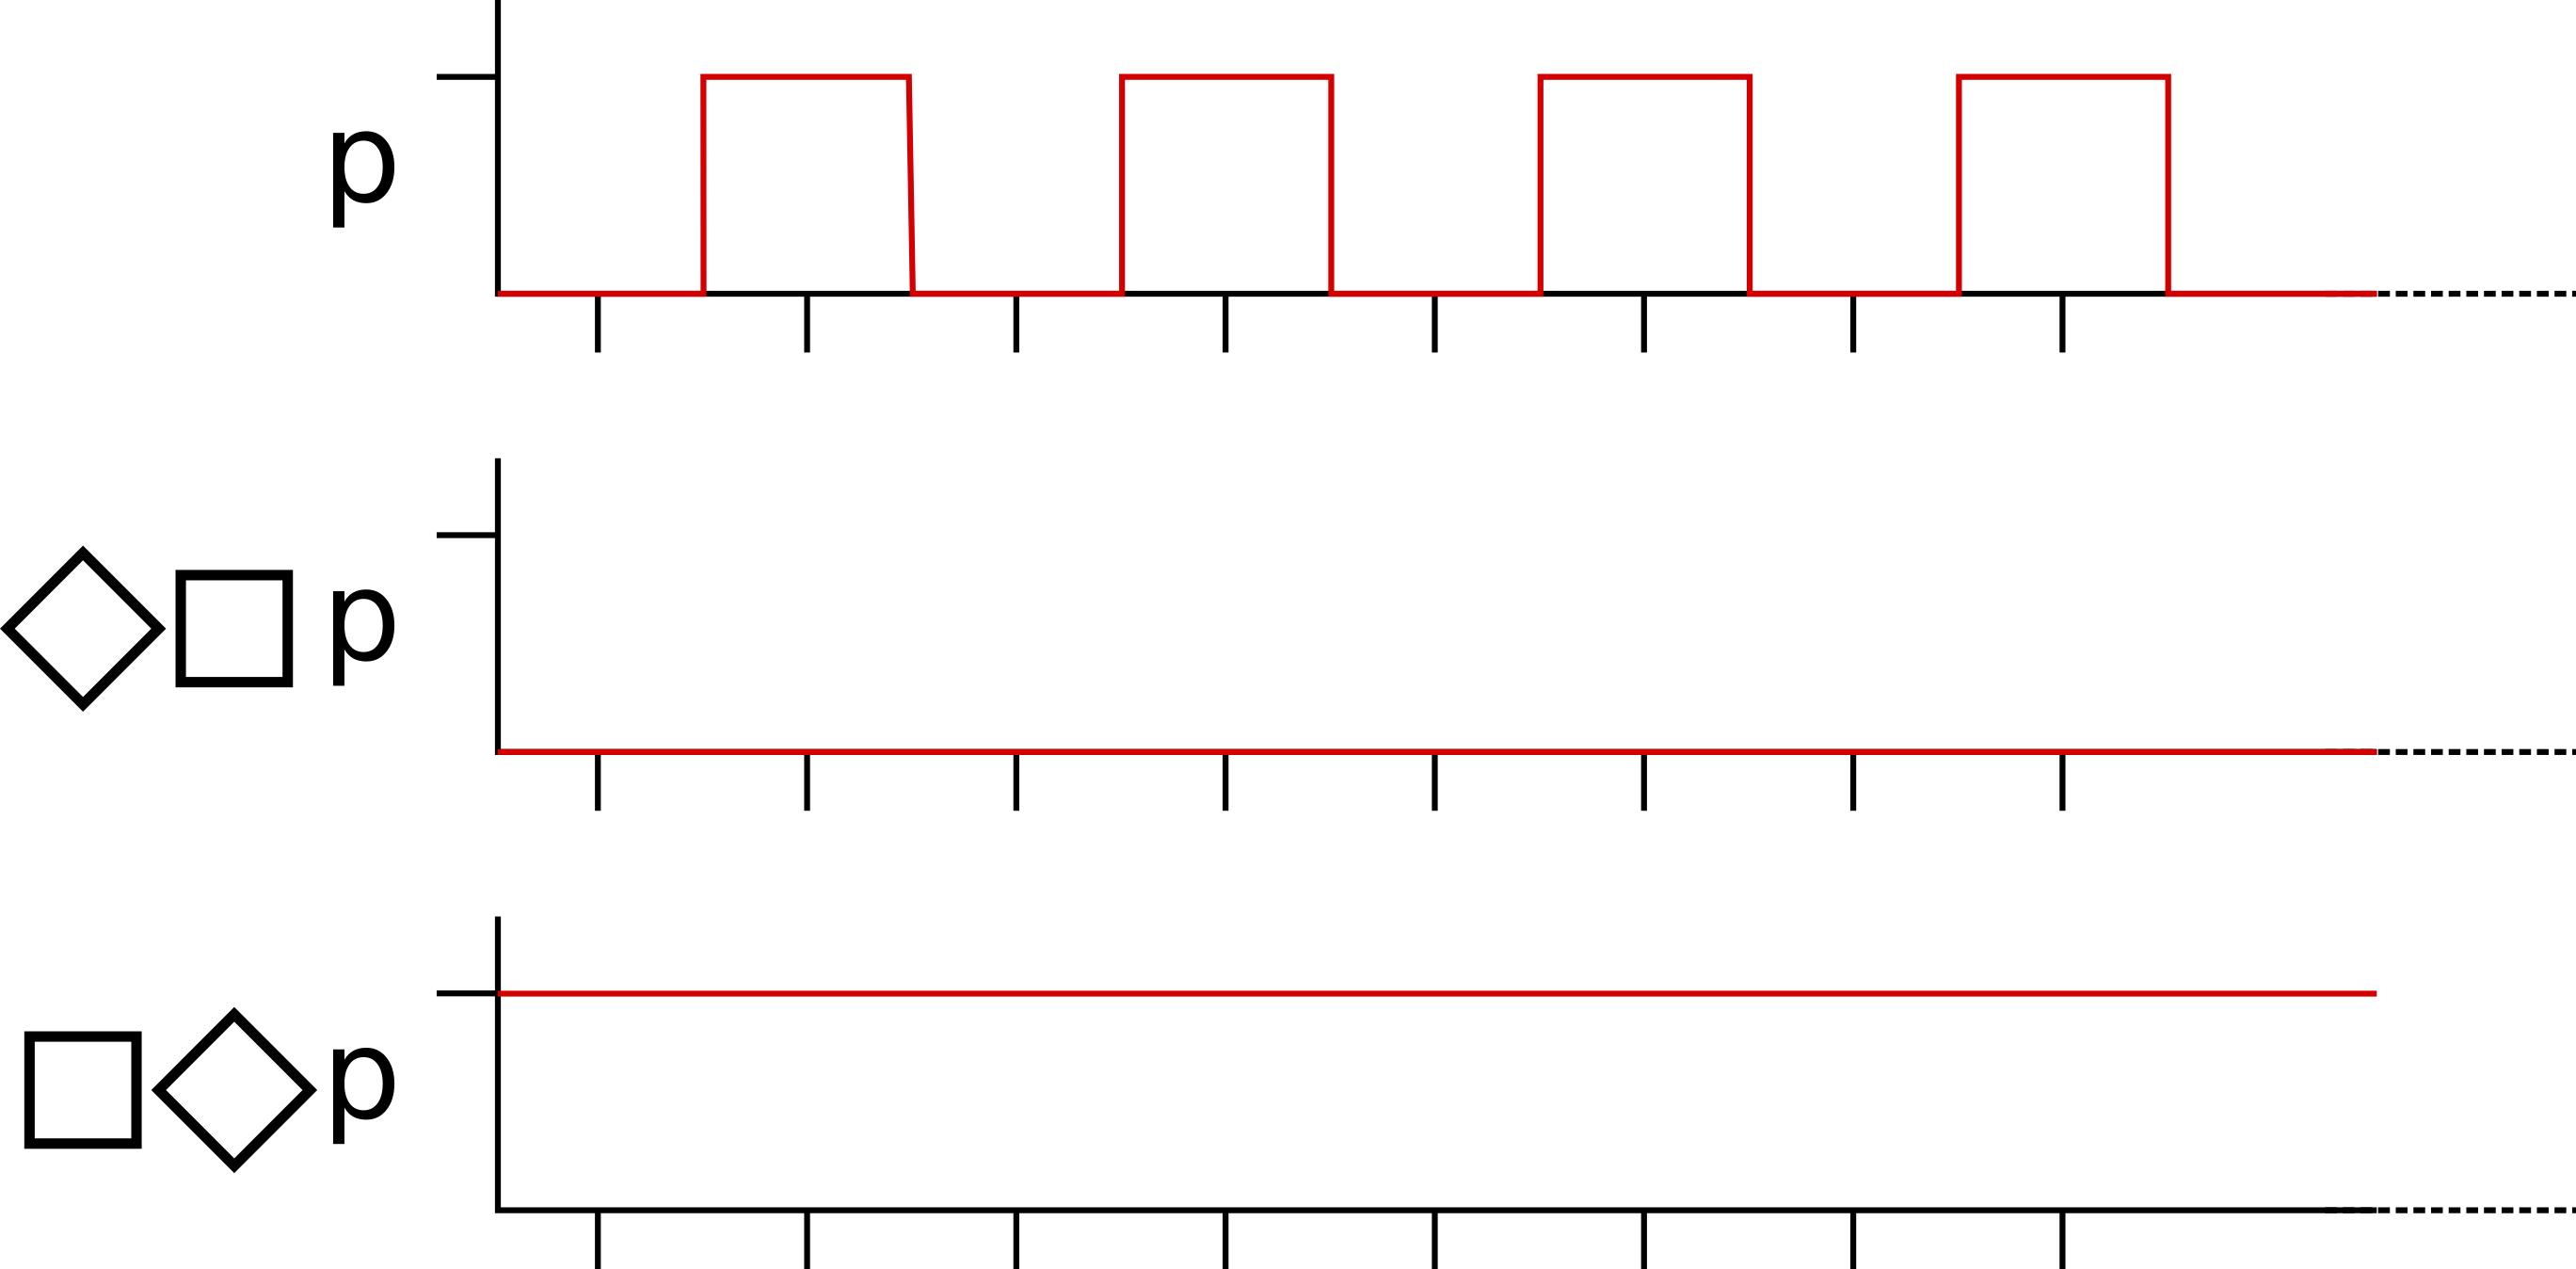
\includegraphics[width=0.5\textwidth]{1_a.png}

Anhand der Grafik l"asst sich erkennen, dass die Aussage nicht f"ur alle Belegungen gilt.

  \item \begin{eqnarray}
		     ((\Box\, p \Rightarrow \lozenge\, q) \land \lozenge \Box\, q )& \Rightarrow & \lozenge\, q
		\end{eqnarray}

Die Aussage gilt f"ur alle Belegungen, da die schw"achere Aussage $\lozenge \Box\, q \Rightarrow \lozenge\, q$ f"ur alle Belegungen gilt: Wenn ab einem Zeitpunkt q immer \textit{true} ist, dann ist q auch irgendwann in der Zukunft \textit{true}.

\item
\begin{enumerate}
\item zu Zeigen: $(\Box\, p \wedge \Box\, q) \Leftrightarrow \Box (p \wedge q)$

$
\Box\, p_i \wedge \Box\, q_i := \forall j \geq i : p_j \wedge \forall j \geq i:q_j => \forall j \geq i: p_j \wedge q_j
$

$
\Box (p_i \wedge q_i) := \forall j \geq i: p_j \wedge q_j
$

q.e.d.

\item zu Zeigen: $(\lozenge\, p \vee \lozenge\, q) \Leftrightarrow \lozenge (p \vee q)$

$
\lozenge\, p_i \vee \lozenge\, q_i := \exists j \geq i: p_j \vee \exists j \geq i: q_j => \exists j \geq i: p \vee q
$

$
\lozenge (p \vee q) := \exists j \geq i: p \vee q
$

q.e.d.
\end{enumerate}
\end{enumerate}

% Aufgabe 2
\AUFGABE{Lineare Temporale Logik II}{10 Punkte}
\begin{enumerate}
\item
\begin{enumerate}
\item
$I_x(\alpha U \beta) = I_x(\alpha )\dot{U} I_x(\beta)$ mit $\dot{U}: \{t,f\}^{N x N} \rightarrow \{t,f\}^N$ \\
wobei $\dot{U}((a_i)_{i\in N}, (b_i)_{i\in N}) = (w_i)_{i\in N}$\\
und $w_i = \begin{cases} t & falls\, \exists j\geq i: b_j = t \land \forall k\in [i, ..., j): a_k = t \\ f & sonst \end{cases}$
\begin{figure}
  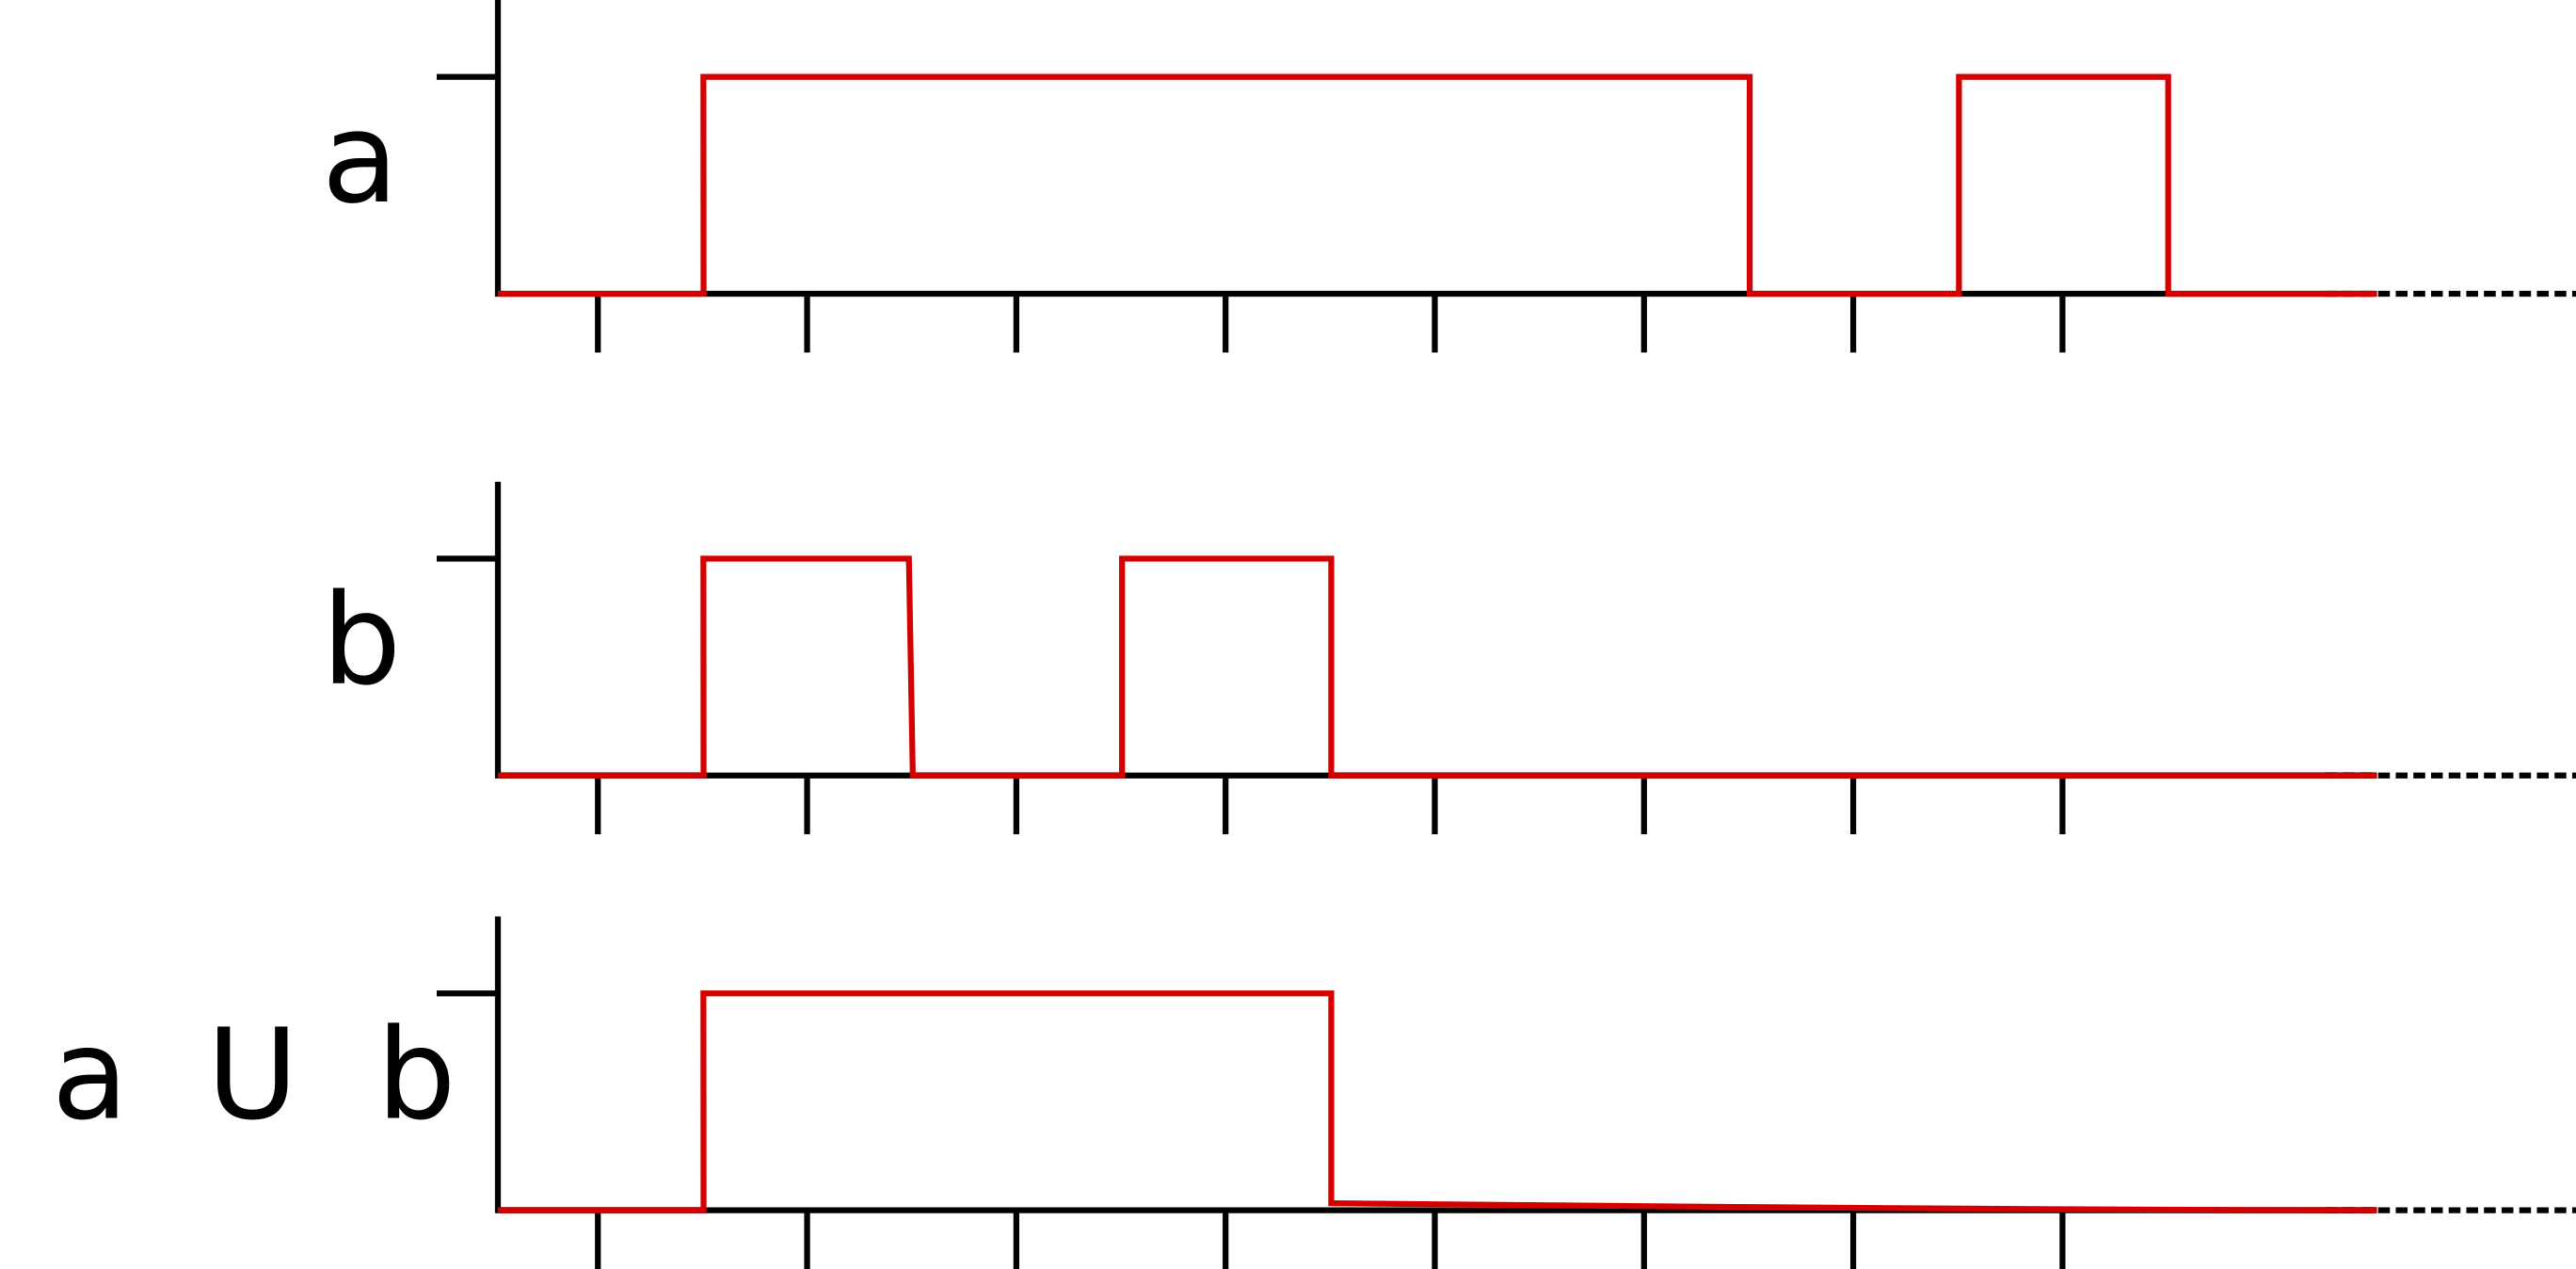
\includegraphics[width=0.5\textwidth]{2_a_1.png}
\caption{Beispiel f"ur den \textit{bis} Operator}
\end{figure}

\item
$I_x(\bigcirc \alpha) = \dot{\bigcirc} I_x(\alpha )$ mit $\dot{\bigcirc}: \{t,f\}^N \rightarrow \{t,f\}^N$ \\
wobei $\dot{\bigcirc}((a_i)_{i\in N}) = (w_i)_{i\in N}$\\
und $w_i = \begin{cases}
 t, & falls\, a_{i+1} = t\\
 f, & sonst
 \end{cases}$
 	\begin{figure}
 	   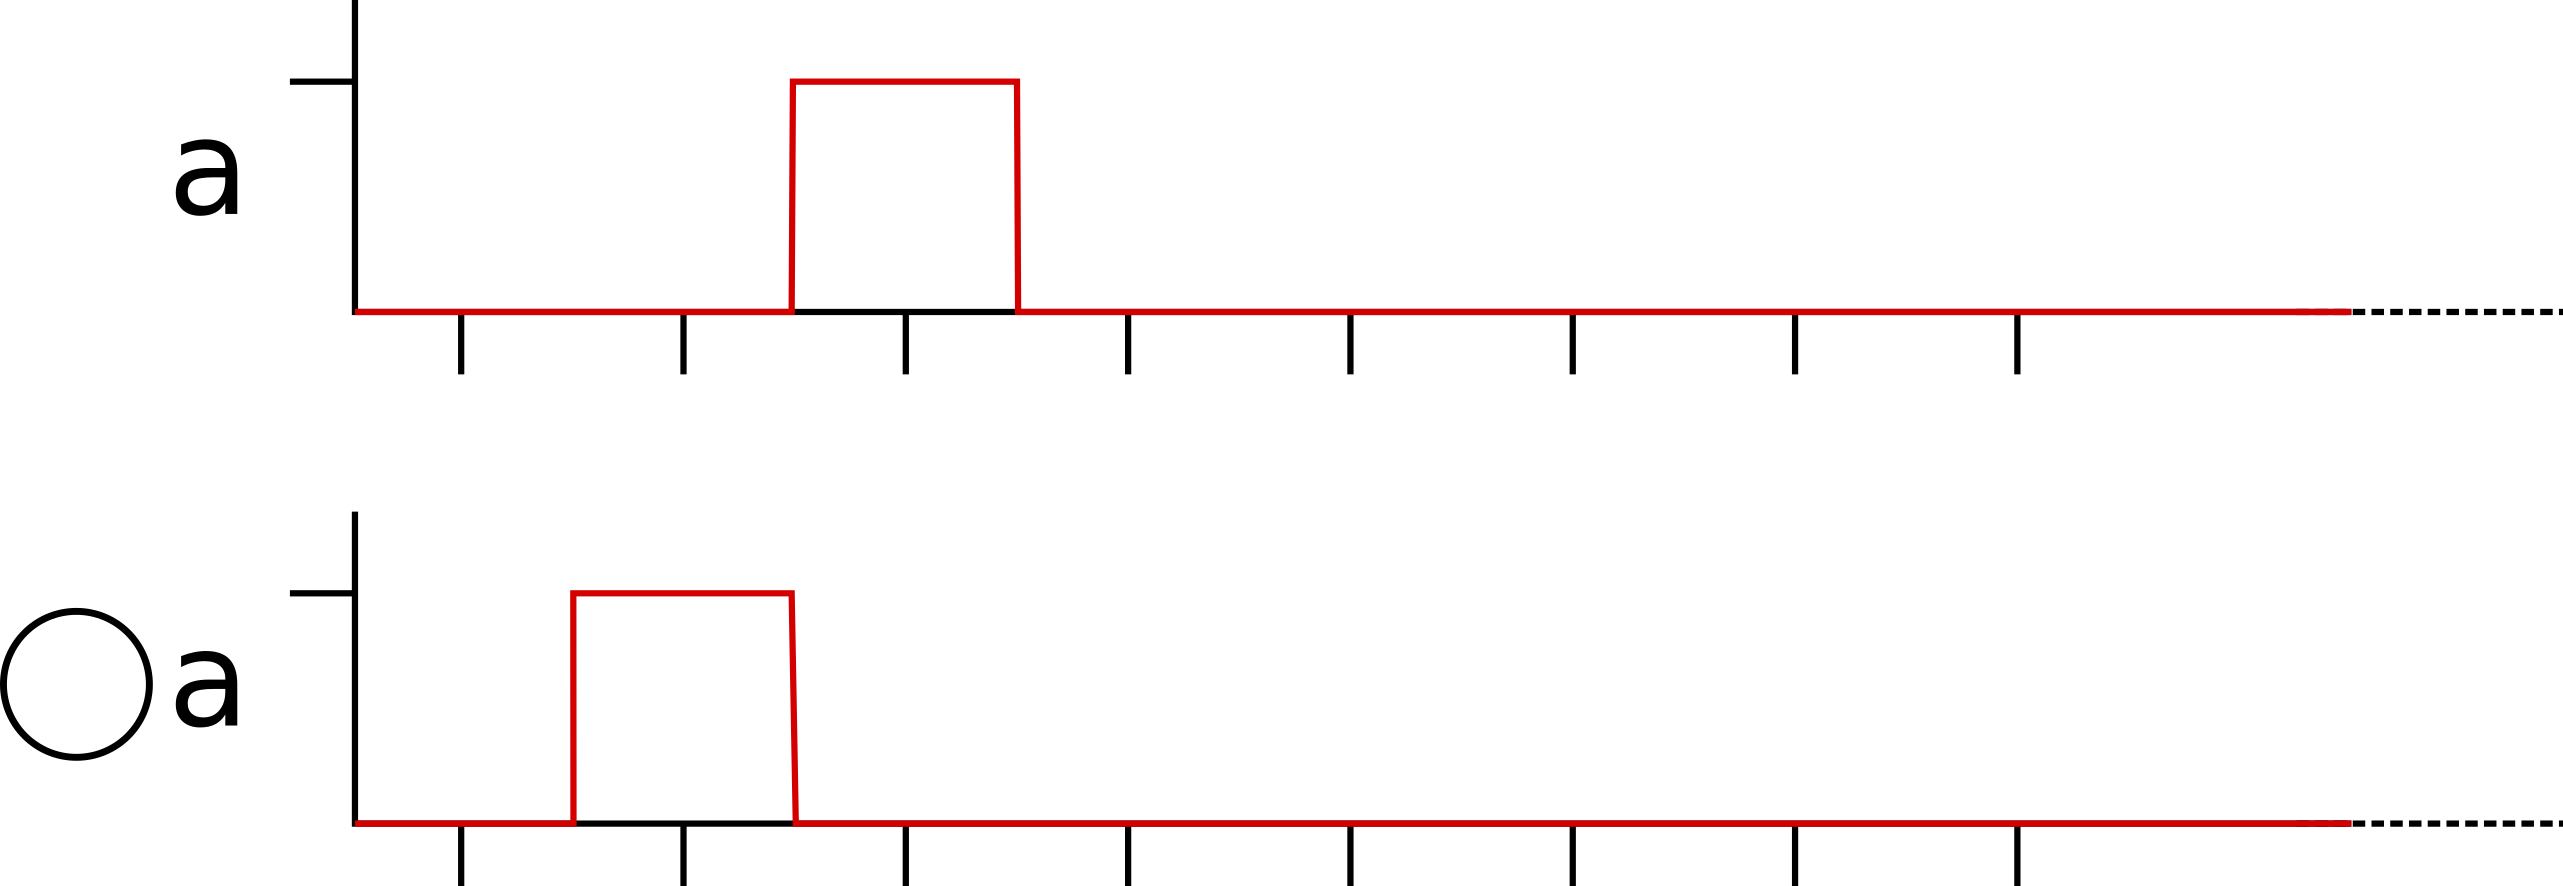
\includegraphics[width=0.5\textwidth]{2_a_2.png}
	\caption{Beispiel f"ur den \textit{n"achster} Operator}
 	\end{figure}

\end{enumerate}

\item
Falls mehrere Threads im Spiel sind, ist der n"achste Schritt unter Annahme schwacher Fairness nicht genau definiert.

\item
$ \lozenge\, a \equiv true\, Ua$, da letzteres true ist, wenn $\exists j\geq i: a_j = true \land true $\\

$ \Box\, a \equiv \neg (\lozenge\, (\neg a)) \equiv \neg (true\, U\neg a)$, die Herleitung folgt dementsprechend aus dem 1. Fall.\\

\end{enumerate}

% Aufgabe 1
\AUFGABE{Der Algorthmus von Peterson II}{10 Punkte}
\begin{verbatim}
======================================================
  global adrin = false, bdrin = false, letzter = a
a1: U                     | b1: U
a2: adrin  <- true        | b2: bdrin  <- true
a3: letzter <- a          | b3: letzter <- b
a4: while bdrin &&        | b4: while adrin &&
          letzter = a do  |           letzter = b do
a5:     NOP               | b5:     NOP
a6: K                     | b6: K
a7: adrin <- false        | b7: bdrin <- false
\end{verbatim}
F"ur alle m"oglichen Zustandsfolgen gilt:
\begin{itemize}
	\item $\immer(a_1 \folgt \irgendwann (a_2 \oder a_\bot))$
	\item $\immer(a_2 \folgt \irgendwann a_3)$
	\item $\immer(a_3 \folgt \irgendwann a_4)$
	\item $\immer(a_4 \folgt \irgendwann (a_5 \oder a_6)$
	\item $\immer(a_5 \folgt \irgendwann a_4)$
	\item $\immer(a_6 \folgt \irgendwann a_7)$
	\item $\immer(a_7 \folgt \irgendwann a_1)$
	\item $\immer(a_\bot \folgt \immer a_\bot)$
	\item Analog f"ur die Zust"ande von $b$
\end{itemize}

Au"serdem legen wir folgende Invarianten fest:
\begin{enumerate}
	\item[1)] $\immer(letzter = a \oder letzter = b)$
	\item[2)] $\immer(adrin \equiv a_3 \oder a_4 \oder a_5 \oder a_6 \oder a_7)$
	\item[3)] $\immer(bdrin \equiv b_3 \oder b_4 \oder b_5 \oder b_6 \oder b_7)$
\end{enumerate}

\begin{enumerate}
	\item Zu beweisen:
	\begin{itemize}
		\item $(a_6 \und (b_4 \oder b_5)) \folgt (adrin \und letzter = b)$\\
			Beweis durch Widerspruch:
			\[ \neg((a_6 \und (b_4 \oder b_5)) \folgt (adrin \und letzter = b)) \]
			\[ (a_6 \und (b_4 \oder b_5)) \und \neg (adrin \und letzter = b) \]
			\[ (a_6 \und (b_4 \oder b_5)) \und (\neg adrin \oder letzter \neq b) \]
			Aus Invariante 1) folgt:
			\[ (a_6 \und (b_4 \oder b_5)) \und (\neg adrin \oder letzter = a) \]
			Nach Invariante 2) und $a_6$ ist $adrin = true$:
			\[ (a_6 \und (b_4 \oder b_5)) \und (false \oder letzter = a) \]
			\[ a_6 \und (b_4 \oder b_5) \und letzter = a \]
			Aus $(b_4 \oder b_5)$ und Invariante 3) folgt $bdrin = true$\\
			$b$ befindet sich in der Schleife, wartet also darauf dass $a$
			$adrin$ auf $false$ setzt. Ist aber $letzter = a$ und $bdrin = true$,
			so h"atte $a$ niemals von $a_4$ nach $a_6$ gehen d"urfen.

			Folglich kann nicht gleichzeitig $a_6$, $(b_4 \oder b_5)$ und $letzter = a$ gelten:\\
			\emph{Widerspruch!}

		\item $((a_4 \oder a_5) \und b_6) \folgt (bdrin \und letzter = a)$\\
			Beweis analog zu vorherigem, nur mit $a$ und $b$ vertauscht.
	\end{itemize}
	\item Zu zeigen:
	\begin{itemize}
		\item $\immer \big [(a_4 \und \immer \neg a_6) \folgt \immer \irgendwann (bdrin \und letzter \neq b) \big ]$

		Invariante 1): $letzter \neq b \equiv letzter = a$
		\[ \immer \big [(a_4 \und \immer \neg a_6) \folgt \immer \irgendwann (bdrin \und letzter = a) \big ] \]
		Es gilt immer, dass, wenn $a$ einerseits bei $a_4$, also vor bei der "Uberpr"ufung der Schleife ist,
		andererseits \emph{niemals}(immer nicht) $a_6$ eintreten wird, daraus folgt, dass immer
		irgendwann $bdrin = true$ und $letzter = a$ sein muss.

		Beweis durch Widerspruch: Nehmen wir an, $a$ ist bei $a_4$ und es wird niemals $a_6$ eintreten,
		irgendwann wird aber $bdrin = false$ oder $letzter \neq a$. Dann k"onnte im Folgenden
		$a$ einen Schritt machen, die Schleifenbedingungen sind nicht erf"ullt und $a$ w"urde von
		$a_4$ in $a_6$ "ubergehen. Dass niemals $a_6$ eintreten kann wurde aber vorausgesetzt:
		\emph{Widerspruch!}

		Formal:
		\[ \neg\left(\immer\left[(a_4\und\immer\neg a_6)\folgt\immer\irgendwann(bdrin\und letzter=a)\right]\right) \]
		\[ \irgendwann\left(\neg\left[(a_4\und\immer\neg a_6)\folgt\immer\irgendwann(bdrin\und letzter=a)\right]\right) \]
		\[ \irgendwann\left[(a_4\und\immer\neg a_6)\und\neg\immer\irgendwann(bdrin\und letzter=a)\right] \]
		\[ \irgendwann\left[(a_4\und\immer\neg a_6)\und\irgendwann\neg\irgendwann(bdrin\und letzter=a)\right] \]
		\[ \irgendwann\left[(a_4\und\immer\neg a_6)\und\irgendwann\immer\neg(bdrin\und letzter=a)\right] \]
		\[ \irgendwann\left[(a_4\und\immer\neg a_6)\und\irgendwann\immer(\neg bdrin\oder letzter\neq a)\right] \]

		Ist nun $bdrin = false$ oder $letzter \neq a$, wird der rechte Teilausdruck zu
		$true$ ausgewertet, der linke Teilausdruck jedoch \emph{irgendwann}(n"amlich wenn $a$ den
		n"achsten Schritt macht) zu $false$, da $a$ dann bei $a_6$ ist, was jedoch \emph{niemals}
		eintreten sollte.

		\item $\immer \big [\irgendwann \immer (\neg bdrin) \oder \irgendwann (letzter = b) \big]$

		Es gilt immer, dass entweder irgendwann immer $bdrin = false$ ist oder dass irgendwann
		$letzter = b$ sein wird.

		Damit $bdrin$ dauerhaft (\emph{immer}) $false$ bleiben w"urde, m"usste $b$ in
		$b_1$ abst"urzen und zu $b_\bot$ "ubergehen, da $bdrin$ nur in $b_1$ und $b_2$
		$false$ ist und wir eingangs gefordert haben, dass immer auf $b_2$ irgendwann
		$b_3$ folgt, wodurch dem $bdrin$ wieder auf $true$ gesetzt werden w"urde. Nur
		wenn $b$ von $a_1$ zu $a_\bot$ "ubergeht, in dem es daraufhin f"ur immer verweilen
		w"urde (siehe ebenfalls aufgestellte Bedingungen), kann $bdrin$ f"ur immer
		$false$ bleiben.

		St"urzt $b$ jedoch nicht ab und geht folglich von $b_1$ zu $b_2$ "uber, wird
		es immer auch irgendwann zu $b_3$ und weiter zu $b_4$ "ubergehen, wonach
		$letzter = b$ gelten w"urde, womit $\irgendwann (letzter = b)$ gelten w"urde.

		Also:
		\[ \irgendwann\immer(\neg bdrin) \equiv b_\bot \]
		Falls $b_\bot$, dann $\irgendwann\immer(\neg bdrin)$,
		sonst $\irgendwann (letzter = b)$

		\item $\immer \big [(a_4 \und \immer \neg a_6 \und \irgendwann (letzter = b)) \folgt \irgendwann \immer (letzter = b)) \big ]$

		% Es gilt immer, dass aus $a_4 \und \immer \neg a_6 \und \irgendwann (letzter = b)$
		% folgt, dass irgendwann $letzter$ f"ur immer $b$ bleibt.
	\end{itemize}
\begin{verbatim}


======================================================
  global adrin = false, bdrin = false, letzter = a
a1: U                     | b1: U
a2: adrin  <- true        | b2: bdrin  <- true
a3: letzter <- a          | b3: letzter <- b
a4: while bdrin &&        | b4: while adrin &&
          letzter = a do  |           letzter = b do
a5:     NOP               | b5:     NOP
a6: K                     | b6: K
a7: adrin <- false        | b7: bdrin <- false
\end{verbatim}
\end{enumerate}

\end{description}
\end{document}